\documentclass[]{article}
\usepackage{lmodern}
\usepackage{amssymb,amsmath}
\usepackage{ifxetex,ifluatex}
\usepackage{fixltx2e} % provides \textsubscript
\ifnum 0\ifxetex 1\fi\ifluatex 1\fi=0 % if pdftex
  \usepackage[T1]{fontenc}
  \usepackage[utf8]{inputenc}
\else % if luatex or xelatex
  \ifxetex
    \usepackage{mathspec}
  \else
    \usepackage{fontspec}
  \fi
  \defaultfontfeatures{Ligatures=TeX,Scale=MatchLowercase}
\fi
% use upquote if available, for straight quotes in verbatim environments
\IfFileExists{upquote.sty}{\usepackage{upquote}}{}
% use microtype if available
\IfFileExists{microtype.sty}{%
\usepackage{microtype}
\UseMicrotypeSet[protrusion]{basicmath} % disable protrusion for tt fonts
}{}
\usepackage[margin=1in]{geometry}
\usepackage{hyperref}
\hypersetup{unicode=true,
            pdftitle={R Markdown},
            pdfauthor={Helio},
            pdfborder={0 0 0},
            breaklinks=true}
\urlstyle{same}  % don't use monospace font for urls
\usepackage{color}
\usepackage{fancyvrb}
\newcommand{\VerbBar}{|}
\newcommand{\VERB}{\Verb[commandchars=\\\{\}]}
\DefineVerbatimEnvironment{Highlighting}{Verbatim}{commandchars=\\\{\}}
% Add ',fontsize=\small' for more characters per line
\usepackage{framed}
\definecolor{shadecolor}{RGB}{248,248,248}
\newenvironment{Shaded}{\begin{snugshade}}{\end{snugshade}}
\newcommand{\AlertTok}[1]{\textcolor[rgb]{0.94,0.16,0.16}{#1}}
\newcommand{\AnnotationTok}[1]{\textcolor[rgb]{0.56,0.35,0.01}{\textbf{\textit{#1}}}}
\newcommand{\AttributeTok}[1]{\textcolor[rgb]{0.77,0.63,0.00}{#1}}
\newcommand{\BaseNTok}[1]{\textcolor[rgb]{0.00,0.00,0.81}{#1}}
\newcommand{\BuiltInTok}[1]{#1}
\newcommand{\CharTok}[1]{\textcolor[rgb]{0.31,0.60,0.02}{#1}}
\newcommand{\CommentTok}[1]{\textcolor[rgb]{0.56,0.35,0.01}{\textit{#1}}}
\newcommand{\CommentVarTok}[1]{\textcolor[rgb]{0.56,0.35,0.01}{\textbf{\textit{#1}}}}
\newcommand{\ConstantTok}[1]{\textcolor[rgb]{0.00,0.00,0.00}{#1}}
\newcommand{\ControlFlowTok}[1]{\textcolor[rgb]{0.13,0.29,0.53}{\textbf{#1}}}
\newcommand{\DataTypeTok}[1]{\textcolor[rgb]{0.13,0.29,0.53}{#1}}
\newcommand{\DecValTok}[1]{\textcolor[rgb]{0.00,0.00,0.81}{#1}}
\newcommand{\DocumentationTok}[1]{\textcolor[rgb]{0.56,0.35,0.01}{\textbf{\textit{#1}}}}
\newcommand{\ErrorTok}[1]{\textcolor[rgb]{0.64,0.00,0.00}{\textbf{#1}}}
\newcommand{\ExtensionTok}[1]{#1}
\newcommand{\FloatTok}[1]{\textcolor[rgb]{0.00,0.00,0.81}{#1}}
\newcommand{\FunctionTok}[1]{\textcolor[rgb]{0.00,0.00,0.00}{#1}}
\newcommand{\ImportTok}[1]{#1}
\newcommand{\InformationTok}[1]{\textcolor[rgb]{0.56,0.35,0.01}{\textbf{\textit{#1}}}}
\newcommand{\KeywordTok}[1]{\textcolor[rgb]{0.13,0.29,0.53}{\textbf{#1}}}
\newcommand{\NormalTok}[1]{#1}
\newcommand{\OperatorTok}[1]{\textcolor[rgb]{0.81,0.36,0.00}{\textbf{#1}}}
\newcommand{\OtherTok}[1]{\textcolor[rgb]{0.56,0.35,0.01}{#1}}
\newcommand{\PreprocessorTok}[1]{\textcolor[rgb]{0.56,0.35,0.01}{\textit{#1}}}
\newcommand{\RegionMarkerTok}[1]{#1}
\newcommand{\SpecialCharTok}[1]{\textcolor[rgb]{0.00,0.00,0.00}{#1}}
\newcommand{\SpecialStringTok}[1]{\textcolor[rgb]{0.31,0.60,0.02}{#1}}
\newcommand{\StringTok}[1]{\textcolor[rgb]{0.31,0.60,0.02}{#1}}
\newcommand{\VariableTok}[1]{\textcolor[rgb]{0.00,0.00,0.00}{#1}}
\newcommand{\VerbatimStringTok}[1]{\textcolor[rgb]{0.31,0.60,0.02}{#1}}
\newcommand{\WarningTok}[1]{\textcolor[rgb]{0.56,0.35,0.01}{\textbf{\textit{#1}}}}
\usepackage{longtable,booktabs}
\usepackage{graphicx,grffile}
\makeatletter
\def\maxwidth{\ifdim\Gin@nat@width>\linewidth\linewidth\else\Gin@nat@width\fi}
\def\maxheight{\ifdim\Gin@nat@height>\textheight\textheight\else\Gin@nat@height\fi}
\makeatother
% Scale images if necessary, so that they will not overflow the page
% margins by default, and it is still possible to overwrite the defaults
% using explicit options in \includegraphics[width, height, ...]{}
\setkeys{Gin}{width=\maxwidth,height=\maxheight,keepaspectratio}
\IfFileExists{parskip.sty}{%
\usepackage{parskip}
}{% else
\setlength{\parindent}{0pt}
\setlength{\parskip}{6pt plus 2pt minus 1pt}
}
\setlength{\emergencystretch}{3em}  % prevent overfull lines
\providecommand{\tightlist}{%
  \setlength{\itemsep}{0pt}\setlength{\parskip}{0pt}}
\setcounter{secnumdepth}{0}
% Redefines (sub)paragraphs to behave more like sections
\ifx\paragraph\undefined\else
\let\oldparagraph\paragraph
\renewcommand{\paragraph}[1]{\oldparagraph{#1}\mbox{}}
\fi
\ifx\subparagraph\undefined\else
\let\oldsubparagraph\subparagraph
\renewcommand{\subparagraph}[1]{\oldsubparagraph{#1}\mbox{}}
\fi

%%% Use protect on footnotes to avoid problems with footnotes in titles
\let\rmarkdownfootnote\footnote%
\def\footnote{\protect\rmarkdownfootnote}

%%% Change title format to be more compact
\usepackage{titling}

% Create subtitle command for use in maketitle
\newcommand{\subtitle}[1]{
  \posttitle{
    \begin{center}\large#1\end{center}
    }
}

\setlength{\droptitle}{-2em}

  \title{R Markdown}
    \pretitle{\vspace{\droptitle}\centering\huge}
  \posttitle{\par}
    \author{Helio}
    \preauthor{\centering\large\emph}
  \postauthor{\par}
      \predate{\centering\large\emph}
  \postdate{\par}
    \date{2020-12-02T10:33:41+09:00}


\begin{document}
\maketitle

\hypertarget{r-markdown}{%
\subsection{R Markdown}\label{r-markdown}}

Este es un documento en formato R Markdown. Markdown es un sintaxis de
formato simple para crear documentos HTML, PDF, y MS Word. Para más
detalles de como utilizar R Markdown visita
\url{http://rmarkdown.rstudio.com}.

Cuando presoinas el botón \textbf{Knit}, se genera un documento que
incluye tanto el contenido como el como el resultado de cualquier trozo
de codigo R incrustado dentro del documento. Se puede incrustar un trozo
de codigo R así:

\hypertarget{carga-de-paquetes-necesarios}{%
\subsubsection{Carga de paquetes
necesarios}\label{carga-de-paquetes-necesarios}}

El siguiente codigo carga los paquetes:

\begin{itemize}
\tightlist
\item
  \textbf{readr:}
\item
  \textbf{mosaic:}
\item
  \textbf{FSA:}
\item
  \textbf{ggplot2:}
\item
  \textbf{readxl:}
\item
  \textbf{knitr:}
\item
  \textbf{doBy:}
\item
  \textbf{agricolae:}
\end{itemize}

\begin{Shaded}
\begin{Highlighting}[]
\KeywordTok{library}\NormalTok{(readr)}
\KeywordTok{library}\NormalTok{(mosaic)}
\KeywordTok{library}\NormalTok{(FSA)}
\KeywordTok{library}\NormalTok{(}\StringTok{"ggplot2"}\NormalTok{)}
\KeywordTok{library}\NormalTok{(readxl)}
\KeywordTok{library}\NormalTok{(knitr)}
\KeywordTok{library}\NormalTok{(doBy)}
\KeywordTok{library}\NormalTok{(agricolae)}
\KeywordTok{options}\NormalTok{(}\DataTypeTok{scipen=}\DecValTok{999}\NormalTok{, }\DataTypeTok{digits =} \DecValTok{0}\NormalTok{)}
\CommentTok{## Load all the libraries needed and the data}
\end{Highlighting}
\end{Shaded}

\hypertarget{carga-de-archivos-necesarios}{%
\subsubsection{Carga de archivos
necesarios}\label{carga-de-archivos-necesarios}}

El siguiente codigo carga los archivos:

\begin{itemize}
\tightlist
\item
  \textbf{read\_excel:}
\end{itemize}

\begin{Shaded}
\begin{Highlighting}[]
\NormalTok{mydata <-}\StringTok{ }\KeywordTok{read_excel}\NormalTok{(}\StringTok{"./data/2016-Solanum-01-11_Isolates(Germplasms).xlsx"}\NormalTok{)}
\end{Highlighting}
\end{Shaded}

\hypertarget{manejo-de-datos}{%
\subsubsection{Manejo de datos}\label{manejo-de-datos}}

Para manipular de manera eficiente los datos de nuestro archivo, es
conveniente realizar subconjuntos de datos con el comando
\textbf{Subset}. Con el siguiente codigo seleccionamos las variables
independientes y de respuesta que analizaremos posteriormente.

\begin{itemize}
\tightlist
\item
  \textbf{Subset:}
\end{itemize}

\begin{Shaded}
\begin{Highlighting}[]
\CommentTok{####Eggs PER PLANT ####}

\NormalTok{Sub.Eggs <-}\StringTok{ }\KeywordTok{subset}\NormalTok{(mydata,}
                   \DataTypeTok{select=}\KeywordTok{c}\NormalTok{(Nger, }
\NormalTok{                            Isolate, }
\NormalTok{                            EggsP) ) }
\CommentTok{##Create a subset of the desire variable}
\end{Highlighting}
\end{Shaded}

\begin{center}\rule{0.5\linewidth}{\linethickness}\end{center}

\hypertarget{estadistica-descriptiva}{%
\subsubsection{Estadística descriptiva}\label{estadistica-descriptiva}}

Para este ejemplo nuestro objetivo es saber si las variables germoplasma
(Nger) y aislado (Isolate) influyen significativamente sobre la variable
numero de huevos por planta (EggsP). El siguiente método ilustra de
manera sencilla como calcular y almacenar las respuestas necesarias para
realizar un reporte de resultados.

En principio, nuestro conjunto de datos se compone de 5 tratamientos en
germoplasma y 11 en aislados. Esto nos permite realizar nuestro análisis
desde dos enfoques: intentar conocer si existe diferencia significativa
entre el numero de huevos de cada aislado que se reprodujo en cada
germoplasma, o si un mismo aislado se reproduce de manera diferente en
cada uno de los germoplasmas. En este post nos enfocaremos en el
primero, el analisis de cuatro tratamientos, germoplasmas, para 11
aislados diferentes.

Dado que nuestro conjunto de datos contiene una etiqueta especifica para
cada tratamiento, podemos hacer buen uso de \emph{Copiar} y
\emph{Pegar}, y \emph{Buscar y Reemplazar}, para ahorrarnos un poco de
trabajo. En este caso, solo necesitamos realizar el analisis para un
aislado, y para el resto de ellos solo reemplazar su etiqueta por la del
siguiente aislado. En futuras entradas se describirá como automatizar
este proceso.

\hypertarget{manejo-de-datos-1}{%
\subsubsection{Manejo de datos}\label{manejo-de-datos-1}}

Para obtener los datos de nuestro primer aislado utilizamos nuevamente
el comando \textbf{subset}, al cual le añadimos el parametro
\textbf{Isolate == ``MIAd''} para seleccionar solo los datos asociados a
la etiqueta \textbf{MIAd} en la columna \textbf{Isolate}, y
seleccionamos los datos de la columna \textbf{Nger} y \textbf{EggsP}. La
siguiente linea indica que los valores de la columna \textbf{Nger} sean
tratados como factores.

\begin{Shaded}
\begin{Highlighting}[]
\CommentTok{####Isolate: MIAd####}

\NormalTok{Sub.Eggs.MIAd <-}\StringTok{ }\KeywordTok{subset}\NormalTok{(Sub.Eggs, Isolate }\OperatorTok{==}\StringTok{ "MIAd"}\NormalTok{, }\DataTypeTok{select=}\KeywordTok{c}\NormalTok{(Nger, EggsP)) }
\NormalTok{Sub.Eggs.MIAd}\OperatorTok{$}\NormalTok{Nger =}\StringTok{ }\KeywordTok{factor}\NormalTok{ (Sub.Eggs.MIAd}\OperatorTok{$}\NormalTok{Nger, }\DataTypeTok{labels=}\KeywordTok{c}\NormalTok{(}\StringTok{"EC"}\NormalTok{, }\StringTok{"TB"}\NormalTok{, }\StringTok{"TE"}\NormalTok{, }\StringTok{"TS"}\NormalTok{, }\StringTok{"TT"}\NormalTok{)) }
\end{Highlighting}
\end{Shaded}

\hypertarget{promedios-y-error-estandar}{%
\subsubsection{Promedios y error
estándar}\label{promedios-y-error-estandar}}

Para reportar resultados es necesario conocer el promedio y el error
estandar de cada uno de los germoplasmas. Para ello, las primeras 5
lineas de codigo se repiten para cada tratamiento. Primero se obtiene el
subconjunto del tratamiento y se almacena en la variable. A partir de
esta variable se calculan el promedio y el error estandar por medio de
los comandos \textbf{mean} y \textbf{se}, del paquete \_\_\_, se
almacenan en su propia variable, y se redondea el valor a dos digitos
(\textbf{round}).

\begin{Shaded}
\begin{Highlighting}[]
\CommentTok{###Descriptive statistics calculation###}
\NormalTok{Sub.Eggs.MIAd.EC <-}\StringTok{ }\KeywordTok{subset}\NormalTok{(Sub.Eggs.MIAd, Nger }\OperatorTok{==}\StringTok{ "EC"}\NormalTok{, }\DataTypeTok{select=}\KeywordTok{c}\NormalTok{(Nger,EggsP))}
\NormalTok{Me.EP.MIAd.EC <-}\StringTok{ }\KeywordTok{mean}\NormalTok{(Sub.Eggs.MIAd.EC}\OperatorTok{$}\NormalTok{EggsP, }\DataTypeTok{na.mr=}\OtherTok{FALSE}\NormalTok{)}
\NormalTok{Me.EP.MIAd.EC <-}\StringTok{ }\KeywordTok{round}\NormalTok{(Me.EP.MIAd.EC, }\DataTypeTok{digits=}\DecValTok{2}\NormalTok{)}
\NormalTok{Se.EP.MIAd.EC <-}\StringTok{ }\KeywordTok{se}\NormalTok{(Sub.Eggs.MIAd.EC}\OperatorTok{$}\NormalTok{EggsP)}
\NormalTok{Se.EP.MIAd.EC <-}\StringTok{ }\KeywordTok{round}\NormalTok{(Se.EP.MIAd.EC, }\DataTypeTok{digits=}\DecValTok{2}\NormalTok{)}

\NormalTok{Sub.Eggs.MIAd.SB <-}\StringTok{ }\KeywordTok{subset}\NormalTok{(Sub.Eggs.MIAd, Nger }\OperatorTok{==}\StringTok{ "TB"}\NormalTok{, }\DataTypeTok{select=}\KeywordTok{c}\NormalTok{(Nger,EggsP))}
\NormalTok{Me.EP.MIAd.TB <-}\StringTok{ }\KeywordTok{mean}\NormalTok{(Sub.Eggs.MIAd.SB}\OperatorTok{$}\NormalTok{EggsP, }\DataTypeTok{na.mr=}\OtherTok{FALSE}\NormalTok{)}
\NormalTok{Me.EP.MIAd.TB <-}\StringTok{ }\KeywordTok{round}\NormalTok{(Me.EP.MIAd.TB, }\DataTypeTok{digits=}\DecValTok{2}\NormalTok{)}
\NormalTok{Se.EP.MIAd.TB <-}\StringTok{ }\KeywordTok{se}\NormalTok{(Sub.Eggs.MIAd.SB}\OperatorTok{$}\NormalTok{EggsP)}
\NormalTok{Se.EP.MIAd.TB <-}\StringTok{ }\KeywordTok{round}\NormalTok{(Se.EP.MIAd.TB, }\DataTypeTok{digits=}\DecValTok{2}\NormalTok{)}

\NormalTok{Sub.Eggs.MIAd.SB <-}\StringTok{ }\KeywordTok{subset}\NormalTok{(Sub.Eggs.MIAd, Nger }\OperatorTok{==}\StringTok{ "TE"}\NormalTok{, }\DataTypeTok{select=}\KeywordTok{c}\NormalTok{(Nger,EggsP))}
\NormalTok{Me.EP.MIAd.TE <-}\StringTok{ }\KeywordTok{mean}\NormalTok{(Sub.Eggs.MIAd.SB}\OperatorTok{$}\NormalTok{EggsP, }\DataTypeTok{na.mr=}\OtherTok{FALSE}\NormalTok{)}
\NormalTok{Me.EP.MIAd.TE <-}\StringTok{ }\KeywordTok{round}\NormalTok{(Me.EP.MIAd.TE, }\DataTypeTok{digits=}\DecValTok{2}\NormalTok{)}
\NormalTok{Se.EP.MIAd.TE <-}\StringTok{ }\KeywordTok{se}\NormalTok{(Sub.Eggs.MIAd.SB}\OperatorTok{$}\NormalTok{EggsP)}
\NormalTok{Se.EP.MIAd.TE <-}\StringTok{ }\KeywordTok{round}\NormalTok{(Se.EP.MIAd.TE, }\DataTypeTok{digits=}\DecValTok{2}\NormalTok{)}

\NormalTok{Sub.Eggs.MIAd.SB <-}\StringTok{ }\KeywordTok{subset}\NormalTok{(Sub.Eggs.MIAd, Nger }\OperatorTok{==}\StringTok{ "TS"}\NormalTok{, }\DataTypeTok{select=}\KeywordTok{c}\NormalTok{(Nger,EggsP))}
\NormalTok{Me.EP.MIAd.TS <-}\StringTok{ }\KeywordTok{mean}\NormalTok{(Sub.Eggs.MIAd.SB}\OperatorTok{$}\NormalTok{EggsP, }\DataTypeTok{na.mr=}\OtherTok{FALSE}\NormalTok{)}
\NormalTok{Me.EP.MIAd.TS <-}\StringTok{ }\KeywordTok{round}\NormalTok{(Me.EP.MIAd.TS, }\DataTypeTok{digits=}\DecValTok{2}\NormalTok{)}
\NormalTok{Se.EP.MIAd.TS <-}\StringTok{ }\KeywordTok{se}\NormalTok{(Sub.Eggs.MIAd.SB}\OperatorTok{$}\NormalTok{EggsP)}
\NormalTok{Se.EP.MIAd.TS <-}\StringTok{ }\KeywordTok{round}\NormalTok{(Se.EP.MIAd.TS, }\DataTypeTok{digits=}\DecValTok{2}\NormalTok{)}

\NormalTok{Sub.Eggs.MIAd.SB <-}\StringTok{ }\KeywordTok{subset}\NormalTok{(Sub.Eggs.MIAd, Nger }\OperatorTok{==}\StringTok{ "TT"}\NormalTok{, }\DataTypeTok{select=}\KeywordTok{c}\NormalTok{(Nger,EggsP))}
\NormalTok{Me.EP.MIAd.TT <-}\StringTok{ }\KeywordTok{mean}\NormalTok{(Sub.Eggs.MIAd.SB}\OperatorTok{$}\NormalTok{EggsP, }\DataTypeTok{na.mr=}\OtherTok{FALSE}\NormalTok{)}
\NormalTok{Me.EP.MIAd.TT <-}\StringTok{ }\KeywordTok{round}\NormalTok{(Me.EP.MIAd.TT, }\DataTypeTok{digits=}\DecValTok{2}\NormalTok{)}
\NormalTok{Se.EP.MIAd.TT <-}\StringTok{ }\KeywordTok{se}\NormalTok{(Sub.Eggs.MIAd.SB}\OperatorTok{$}\NormalTok{EggsP)}
\NormalTok{Se.EP.MIAd.TT <-}\StringTok{ }\KeywordTok{round}\NormalTok{(Se.EP.MIAd.TT, }\DataTypeTok{digits=}\DecValTok{2}\NormalTok{)}
\end{Highlighting}
\end{Shaded}

\hypertarget{kruskalwallis-test}{%
\subsubsection{Kruskal--Wallis test}\label{kruskalwallis-test}}

Una vez obtenidos los valores de promedios y error estandar, podemos
dejarlos de lado y proceder a las pruebas estadisticas. Dado que se sabe
que los datos no pertenecen a una distribucion normal, el analisis
no-paramétrico Kruskall-Wallis se calcula utilizando la función
\textbf{kruskal.test} del paquete \_\_\_\_ (las pruebas de normalidad
las pondré en otra entrada). En este caso, el resultado se guarda en la
variable \emph{KTMIAd}, que será útil más adelante. Para comprender
mejor porqué, se llama a la variable para ver que resultado arroja. Se
observa que tenemos un valor de \emph{P} igual a 0.00007, existe
diferencia significativa entre los tratamientos. La funcion \textbf{ls}
``devuelve un vector de cadenas de caracteres que dan los nombres de los
objetos en el entorno especificado'', y con ella podemos ver que el
valor de \emph{P} se encuentra almacenado bajo el nombre de p.value y
podemos llamarlo mediante \emph{variable\$nombre}.

\begin{Shaded}
\begin{Highlighting}[]
\CommentTok{####Kruskal-Wallis test calculation####}
\NormalTok{KTMIAd =}\StringTok{ }\KeywordTok{kruskal.test}\NormalTok{(Sub.Eggs.MIAd}\OperatorTok{$}\NormalTok{EggsP }\OperatorTok{~}\StringTok{ }\NormalTok{Sub.Eggs.MIAd}\OperatorTok{$}\NormalTok{Nger)}
\NormalTok{KTMIAd}
\end{Highlighting}
\end{Shaded}

\begin{verbatim}
## 
##  Kruskal-Wallis rank sum test
## 
## data:  Sub.Eggs.MIAd$EggsP by Sub.Eggs.MIAd$Nger
## Kruskal-Wallis chi-squared = 30, df = 4, p-value = 0.000007
\end{verbatim}

\begin{Shaded}
\begin{Highlighting}[]
\KeywordTok{ls}\NormalTok{(KTMIAd)}
\end{Highlighting}
\end{Shaded}

\begin{verbatim}
## [1] "data.name" "method"    "p.value"   "parameter" "statistic"
\end{verbatim}

\begin{Shaded}
\begin{Highlighting}[]
\NormalTok{KTMIAd}\OperatorTok{$}\NormalTok{p.value}
\end{Highlighting}
\end{Shaded}

\begin{verbatim}
## [1] 0
\end{verbatim}

\hypertarget{dunns-test}{%
\subsubsection{Dunn's test}\label{dunns-test}}

La prueba anterior indica si existe, o no, diferencia entre los
tratamientos. Para hacer una comparación entre los tratamientos se
utiliza la función \textbf{dunnTest}.

\begin{Shaded}
\begin{Highlighting}[]
\CommentTok{####Dunn test calculation####}
\NormalTok{DTMIAd =}\StringTok{ }\KeywordTok{dunnTest}\NormalTok{(Sub.Eggs.MIAd}\OperatorTok{$}\NormalTok{EggsP }\OperatorTok{~}\StringTok{ }\NormalTok{Sub.Eggs.MIAd}\OperatorTok{$}\NormalTok{Nger, }\DataTypeTok{method=}\StringTok{"bonferroni"}\NormalTok{)}
\KeywordTok{ls}\NormalTok{(DTMIAd)}
\end{Highlighting}
\end{Shaded}

\begin{verbatim}
## [1] "dtres"  "method" "res"
\end{verbatim}

\begin{Shaded}
\begin{Highlighting}[]
\NormalTok{DTMIAd}\OperatorTok{$}\NormalTok{res}
\end{Highlighting}
\end{Shaded}

\begin{verbatim}
##    Comparison  Z P.unadj P.adj
## 1     EC - TB  5       0     0
## 2     EC - TE  3       0     0
## 3     TB - TE -2       0     0
## 4     EC - TS  3       0     0
## 5     TB - TS -2       0     1
## 6     TE - TS  0       1     1
## 7     EC - TT  4       0     0
## 8     TB - TT -2       0     1
## 9     TE - TT  1       1     1
## 10    TS - TT  0       1     1
\end{verbatim}

\begin{Shaded}
\begin{Highlighting}[]
\NormalTok{DTMIAd.Comparison <-}\StringTok{ }\NormalTok{DTMIAd}\OperatorTok{$}\NormalTok{res}\OperatorTok{$}\NormalTok{Comparison}
\NormalTok{DTMIAd.Comparison}
\end{Highlighting}
\end{Shaded}

\begin{verbatim}
##  [1] EC - TB EC - TE TB - TE EC - TS TB - TS TE - TS EC - TT TB - TT
##  [9] TE - TT TS - TT
## 10 Levels: EC - TB EC - TE EC - TS EC - TT TB - TE TB - TS ... TS - TT
\end{verbatim}

\begin{Shaded}
\begin{Highlighting}[]
\NormalTok{DTMIAd.Padj <-}\StringTok{ }\KeywordTok{round}\NormalTok{(DTMIAd}\OperatorTok{$}\NormalTok{res}\OperatorTok{$}\NormalTok{P.adj, }\DataTypeTok{digits=}\DecValTok{5}\NormalTok{)}
\NormalTok{DTMIAd.Padj}
\end{Highlighting}
\end{Shaded}

\begin{verbatim}
##  [1] 0 0 0 0 1 1 0 1 1 1
\end{verbatim}

\begin{Shaded}
\begin{Highlighting}[]
\NormalTok{KrusData =}\StringTok{ }\KeywordTok{data.frame}\NormalTok{(DTMIAd.Comparison, DTMIAd.Padj)}
\NormalTok{KrusData}
\end{Highlighting}
\end{Shaded}

\begin{verbatim}
##    DTMIAd.Comparison DTMIAd.Padj
## 1            EC - TB           0
## 2            EC - TE           0
## 3            TB - TE           0
## 4            EC - TS           0
## 5            TB - TS           1
## 6            TE - TS           1
## 7            EC - TT           0
## 8            TB - TT           1
## 9            TE - TT           1
## 10           TS - TT           1
\end{verbatim}

\begin{Shaded}
\begin{Highlighting}[]
\NormalTok{RND =}\StringTok{ }\KeywordTok{nrow}\NormalTok{(DTMIAd}\OperatorTok{$}\NormalTok{res)}
\NormalTok{RND  }
\end{Highlighting}
\end{Shaded}

\begin{verbatim}
## [1] 10
\end{verbatim}

\begin{Shaded}
\begin{Highlighting}[]
\NormalTok{krustable=}\KeywordTok{kable}\NormalTok{(KrusData[}\DecValTok{1}\OperatorTok{:}\NormalTok{RND,])}
\NormalTok{krustable}
\end{Highlighting}
\end{Shaded}

\begin{longtable}[]{@{}lr@{}}
\toprule
DTMIAd.Comparison & DTMIAd.Padj\tabularnewline
\midrule
\endhead
EC - TB & 0\tabularnewline
EC - TE & 0\tabularnewline
TB - TE & 0\tabularnewline
EC - TS & 0\tabularnewline
TB - TS & 1\tabularnewline
TE - TS & 1\tabularnewline
EC - TT & 0\tabularnewline
TB - TT & 1\tabularnewline
TE - TT & 1\tabularnewline
TS - TT & 1\tabularnewline
\bottomrule
\end{longtable}

\begin{Shaded}
\begin{Highlighting}[]
\NormalTok{DTMIAd}\OperatorTok{$}\NormalTok{dtres}
\end{Highlighting}
\end{Shaded}

\begin{verbatim}
##  [1] "  Kruskal-Wallis rank sum test"                                                 
##  [2] ""                                                                               
##  [3] "data: x and g"                                                                  
##  [4] "Kruskal-Wallis chi-squared = 29.3877, df = 4, p-value = 0"                      
##  [5] ""                                                                               
##  [6] ""                                                                               
##  [7] "                             Comparison of x by g                              "
##  [8] "                                 (Bonferroni)                                  "
##  [9] "Col Mean-|"                                                                     
## [10] "Row Mean |         EC         TB         TE         TS"                         
## [11] "---------+--------------------------------------------"                         
## [12] "      TB |   5.264338"                                                          
## [13] "         |    0.0000*"                                                          
## [14] "         |"                                                                     
## [15] "      TE |   3.020269  -2.244068"                                               
## [16] "         |    0.0253*     0.2483"                                               
## [17] "         |"                                                                     
## [18] "      TS |   3.496750  -1.767587   0.476480"                                    
## [19] "         |    0.0047*     0.7713     1.0000"                                    
## [20] "         |"                                                                     
## [21] "      TT |   3.588972  -1.675365   0.568702   0.092221"                         
## [22] "         |    0.0033*     0.9386     1.0000     1.0000"                         
## [23] ""                                                                               
## [24] "alpha = 0"                                                                      
## [25] "Reject Ho if p <= alpha"
\end{verbatim}

\hypertarget{resultados}{%
\subsubsection{Resultados}\label{resultados}}

El siguiente codigo da una respuesta u otra dependiendo si el valor de P
calculado por la prueba de Kruskal-Wallis es mayor o menor a 0.5.

\begin{Shaded}
\begin{Highlighting}[]
\ControlFlowTok{if}\NormalTok{ (KTMIAd}\OperatorTok{$}\NormalTok{p.value}\OperatorTok{>}\FloatTok{0.05}\NormalTok{) \{}
\NormalTok{dif=}\StringTok{"Existe diferencia significativa entre los tratamientos (P<0.05)"}
\NormalTok{krustable=}\StringTok{"0"}
\NormalTok{\} }\ControlFlowTok{else}\NormalTok{ \{}
\NormalTok{dif=}\StringTok{"No existe diferencia significativa entre los tratamientos (P<0.05)."}
\NormalTok{krustable=}\KeywordTok{kable}\NormalTok{(KrusData[}\DecValTok{1}\OperatorTok{:}\NormalTok{RND,])}
\NormalTok{\}}
\NormalTok{dif}
\end{Highlighting}
\end{Shaded}

\begin{verbatim}
## [1] "No existe diferencia significativa entre los tratamientos (P<0.05)."
\end{verbatim}

No existe diferencia significativa entre los tratamientos
(P\textless{}0.05).

\begin{longtable}[]{@{}lr@{}}
\toprule
DTMIAd.Comparison & DTMIAd.Padj\tabularnewline
\midrule
\endhead
EC - TB & 0\tabularnewline
EC - TE & 0\tabularnewline
TB - TE & 0\tabularnewline
EC - TS & 0\tabularnewline
TB - TS & 1\tabularnewline
TE - TS & 1\tabularnewline
EC - TT & 0\tabularnewline
TB - TT & 1\tabularnewline
TE - TT & 1\tabularnewline
TS - TT & 1\tabularnewline
\bottomrule
\end{longtable}

\hypertarget{reporte-de-resultados}{%
\subsubsection{Reporte de resultados}\label{reporte-de-resultados}}

Con los datos almacenados en variables podemos hacer una tabla como la
siguiente.

\begin{longtable}[]{@{}lll@{}}
\toprule
Germ & Promedio ± Error & Dif\tabularnewline
\midrule
\endhead
EC: & 31517 ± 7491 & a\tabularnewline
TB: & 65 ± 25 & b\tabularnewline
TE: & 360 ± 106 & b\tabularnewline
TS: & 1328 ± 538 & b\tabularnewline
TT: & 220 ± 45 & b\tabularnewline
\bottomrule
\end{longtable}

\begin{center}\rule{0.5\linewidth}{\linethickness}\end{center}

\hypertarget{graficos-generador-por-r}{%
\subsubsection{Graficos generador por
R}\label{graficos-generador-por-r}}

También se pueden incluir graficos. Por ejemplo, la función
\textbf{boxplot}.

\begin{Shaded}
\begin{Highlighting}[]
\KeywordTok{boxplot}\NormalTok{(Sub.Eggs.MIAd}\OperatorTok{$}\NormalTok{EggsP }\OperatorTok{~}\StringTok{ }\NormalTok{Sub.Eggs.MIAd}\OperatorTok{$}\NormalTok{Nger, }\DataTypeTok{main =} \StringTok{"MIAd"}\NormalTok{, }\DataTypeTok{xlab =} \StringTok{"Germplasm"}\NormalTok{, }\DataTypeTok{ylab =} \StringTok{"Eggs per plant"}\NormalTok{)}
\end{Highlighting}
\end{Shaded}

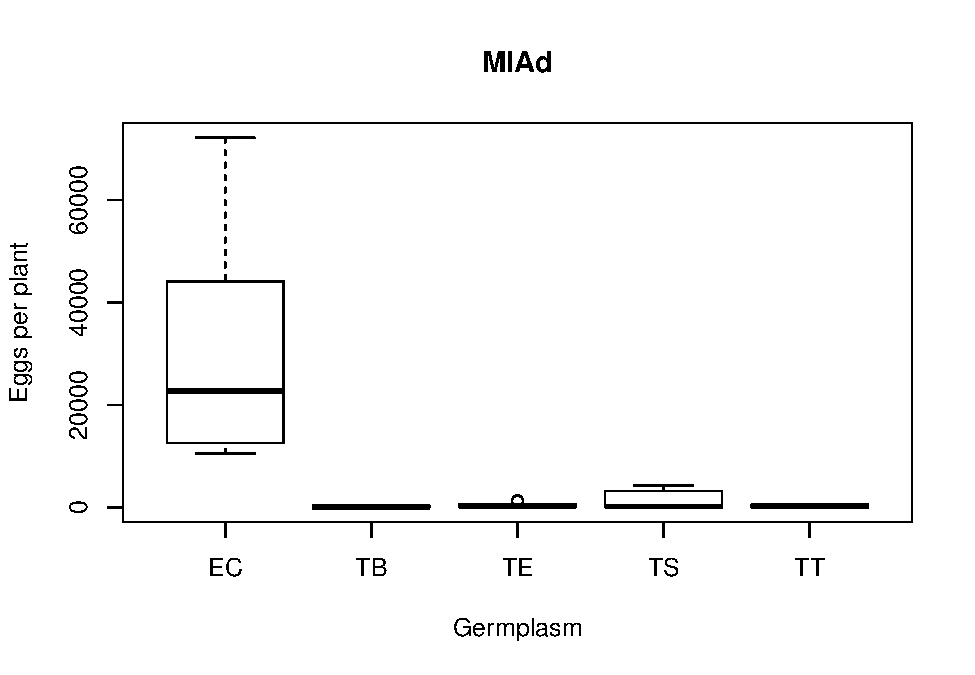
\includegraphics{Post-en-archivo-RMD_files/figure-latex/pressure-1.pdf}

\hypertarget{graficos-no-generados-por-r}{%
\subsubsection{Graficos no generados por
R}\label{graficos-no-generados-por-r}}

Si se desea incluir graficos que no son generados por codigo R, puedes
usar la función \textbf{knitr::include\_graphics()}, la cual te da mas
control sobre los atributos de la imagen que la sintaxis\ldots{} (por
ejemplo, puedes especificar el ancho de la figura mediante out.width).
La figura @ref(fig:Figure01) provee un ejemplo de ello.

\begin{Shaded}
\begin{Highlighting}[]
\NormalTok{knitr}\OperatorTok{::}\KeywordTok{include_graphics}\NormalTok{(}\KeywordTok{rep}\NormalTok{(}\StringTok{'/images/nuevas/20201205_Prueba_RMD01.png'}\NormalTok{, }\DecValTok{1}\NormalTok{)) }\CommentTok{## codigo para Hugo}
\end{Highlighting}
\end{Shaded}

\begin{figure}

{\centering 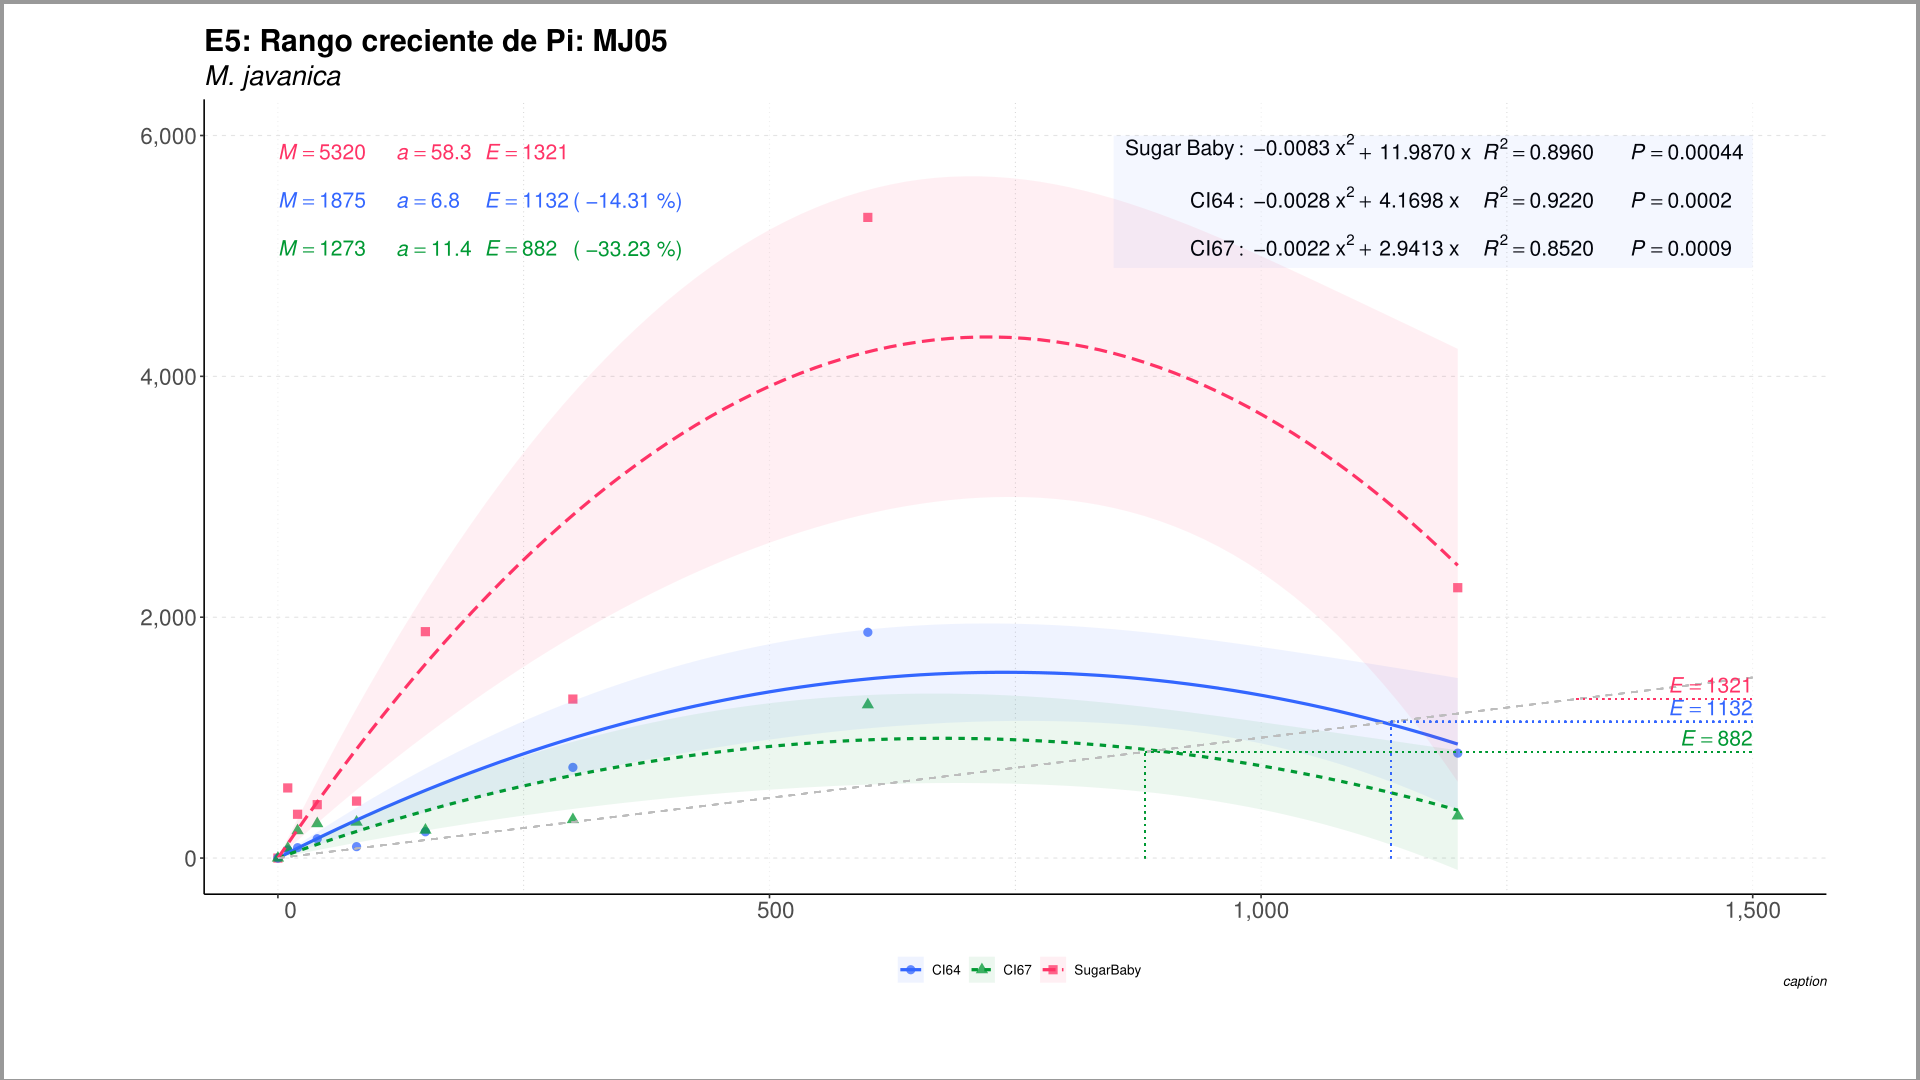
\includegraphics[width=0.9\linewidth]{/images/nuevas/20201205_Prueba_RMD01} 

}

\caption{Figure caption}\label{fig:Figure01}
\end{figure}

El codigo anterior permite generar el siguiente documento en formato
PDF.

\begin{Shaded}
\begin{Highlighting}[]
\NormalTok{knitr}\OperatorTok{::}\KeywordTok{include_url}\NormalTok{(}\KeywordTok{rep}\NormalTok{(}\StringTok{"https://drive.google.com/file/d/1WVU3wqwyk9sTKjaFwtysoLS3uFDiyrae/preview"}\NormalTok{, }\DecValTok{1}\NormalTok{))}
\end{Highlighting}
\end{Shaded}

Figure caption

\hypertarget{chat-de-disqus}{%
\subsubsection{Chat de Disqus}\label{chat-de-disqus}}

\hypertarget{disqus_thread}{}

Please enable JavaScript to view the comments powered by Disqus.


\end{document}
